\documentclass[11pt,a4paper]{article}
\usepackage[czech]{babel}
\usepackage[utf8]{inputenc}
\usepackage{amsmath}
\usepackage{float} %kvůli umístění tabulek a podobně.
%\usepackage[]{mcode} %pro matlabovský kód
\usepackage{etoolbox} %kvůli strequal v newcommand



\usepackage[czech]{babel}
\usepackage[utf8]{inputenc}

\usepackage{graphicx}	%kvůli pdf souboru z MATLABu
\usepackage{setspace}	%rozteče v maticích
\usepackage{verbatim}   %víceřádkové komentáře
\usepackage{siunitx}	%hezký jednotky

\sisetup{locale = DE} % kvůli desetinné čárce (př. v siunits.)


% === Formát stránky ===
\usepackage[a4paper]{geometry}
\geometry{
	verbose,
	tmargin=2.2cm,
	bmargin=1.5cm,
	lmargin=1.5cm,
	rmargin=1.5cm}


\title{%
  Laboratorní úloha - modelovací část\\
  \large Rotační kyvadlo}
\author{Tomáš Glabazňa, Matouš Vrba}
\date{\today}

\begin{document}
\maketitle

\clearpage



%Tomáš%%%%%%%%%%%%%%%%%%%%%%%%%%%%%%%


\section{Rovnice}
\renewcommand{\u}{u}
\newcommand{\x}[2][]{ %první argument je nepovinný, tj. v těchto závorkách []. Pokud to je [t], tak se ta proměnná zobrazí jako funkce času
  \ifstrequal{#1}{t} %podmínka - pokud je první volitelná argument t
   	{x_{#2}(t)} % pak udělej toto
    {x_{#2}}    % jinak udělej toto
}
\newcommand{\xd}[2][]{
  \ifstrequal{#1}{t} 
   	{\dot{x}_{#2}(t)}
    {\dot{x}_{#2}}
}
\newcommand{\y}[1]{y_{#1}}
\newcommand{\M}[1][]{
	\ifstrequal{#1}{t}
	{M(t)}
	{M}
}
\newcommand{\ku}{k_{u}}
\newcommand{\un}{u_{norm}}
\newcommand{\phid}[2][]{
	\ifstrequal{#1}{t}
	{\dot{\varphi}_{#2}(t)}
	{\dot{\varphi}_{#2}}
	}
\newcommand{\phidd}[1]{\ddot{\varphi}_{#1}}
\newcommand{\phin}[2][]{ %phi normální (nederivované)
	\ifstrequal{#1}{t}	
	{\varphi_{#2}(t)}
	{\varphi_{#2}}
	}
\newcommand{\coss}[1]{\cos{(#1)}}
\newcommand{\sinn}[1]{\sin{(#1)}}
\newcommand{\sinnN}[1]{\sin^2{(#1)}} %N = nadruhou

Při popisu systému jsme vycházeli z rovnic popsaných v zadání simulační úlohy. Význam všech zde nedefinovaných proměnných je v něm možné dohledat.

Stavy systému jsme si zvolili jako:
\begin{align*}
& \x{1} = \phin[t]{m}		 && 		\x{2} = \phin[t]{p} \\
& \x{3} = \phid[t]{m}		 &&		\x{4} = \phid[t]{p} \\
\end{align*}

Výstupy jsme definovali jako:
\begin{align*}
& \y{1} = \phin[t]{m}		 &&		\y{2} = \phin[t]{p} \\
\end{align*}

vstup $\u$ pak:
$$
\u = \M[t] = \ku \un
$$
, kde $\un$ je číselný vtup rozhraní k modelu v MATLABu, který je normovaný. $k_u$ je konstanta vyjadřující předpokládanou lineární závislost $\M$ na $\un$.

Stavové rovnice jsou tedy:

\begin{align*}
& \xd{1} = \phid{m}    &&	\xd{2} = \phid{p} \\
\end{align*}
\begin{figure}[H]
\vspace*{-1.3 cm}
$$
\xd{3} =
\frac{
	-J_p k_2 \coss{\x{2}} \x{4}^2 + 2 \delta k_2 \sinn{\x{2}} \x{4} - J_p \M + J_p b \x{3} 	+ k_2 k_3 \coss{\x{2}} \sinn{\x{2}}
}{
 	-J_p k_1 + k_2^2 \sinnN{\x{2}}
}
$$
$$
\xd{4} =
\frac{
	2 \delta \x{4} + k_3 \coss{\x{2}} - \frac{k_2^2}{k_1} \sinn{\x{2}} \coss{\x{2}} 			 	\x{4}^2 - \frac{k_2}{k_1} \sinn{\x{2}} M + \frac{k_2 b}{k_1} \sinn{\x{2}} \x{3}
}{
	-J_p + \frac{k_2^2}{k_1} \sinnN{\x{2}}
}
$$
\end{figure}
\begin{figure}[H]
\vspace*{-1.3 cm}
\begin{align*}
& \y{1} = \x{1}			 &&		\y{2} = \x{2} \\
\end{align*}
\end{figure}

, kde pro konstanty $k_1$, $k_2$ a $k_3$ platí:
$$
k_1 = J_m + m r^2
$$
$$
k_2 = m l r
$$
$$
k_3 = m g l
$$

%Tomáš - konec %%%%%%%%%%%%%%%%%%%%%%%%%%%%%%%




%Matouš%%%%%%%%%%%%%%%%%%%%%%%%%%%%%%%%%%%%%%%%

\section{Linearizace modelu}
Stabilní rovnovážná poloha kyvadla je v pracovním bodě $\mathbf{x_0} = [x_{1p}, x_{2p}, x_{3p}, x_{4p}] = [0, -\frac{\pi}{2}, 0, 0]$, ${u_0} = 0$.
\newline
Matice linearizovaného systému v pracovním bodě $\mathbf{x_0}, u_0$:

\renewcommand{\arraystretch}{1.3}
{\Large
\begin{align*}
&A = 
\begin{pmatrix}
\frac{\partial x_1}{\partial x_1} & \frac{\partial x_1}{\partial x_2} & \frac{\partial x_1}{\partial x_3} & \frac{\partial x_1}{\partial x_4}	\\
\frac{\partial x_2}{\partial x_1} & \frac{\partial x_2}{\partial x_2} & \frac{\partial x_2}{\partial x_3} & \frac{\partial x_2}{\partial x_4}	\\
\frac{\partial x_3}{\partial x_1} & \frac{\partial x_3}{\partial x_2} & \frac{\partial x_3}{\partial x_3} & \frac{\partial x_3}{\partial x_4}	\\
\frac{\partial x_4}{\partial x_1} & \frac{\partial x_4}{\partial x_2} & \frac{\partial x_4}{\partial x_3} & \frac{\partial x_4}{\partial x_4}
\end{pmatrix}_{\biggr\rvert_\mathbf{x_0}} =
\left(\begin{array}{cccc} 0 & 0 & 1 & 0\\ 0 & 0 & 0 & 1\\ 0 & \frac{\mathrm{k_2}\, \mathrm{k_3}}{\mathrm{J_p}\, \mathrm{k_1} - {\mathrm{k_2}}^2} & -\frac{\mathrm{J_p}\, b}{\mathrm{J_p}\, \mathrm{k_1} - {\mathrm{k_2}}^2} & \frac{2\, \mathrm{\delta}\, \mathrm{k_2}}{\mathrm{J_p}\, \mathrm{k_1} - {\mathrm{k_2}}^2}\\ 0 & -\frac{\mathrm{k_3}}{\mathrm{J_p} - \frac{{\mathrm{k_2}}^2}{\mathrm{k_1}}} & \frac{b\, \mathrm{k_2}}{\mathrm{k_1}\, \left(\mathrm{J_p} - \frac{{\mathrm{k_2}}^2}{\mathrm{k_1}}\right)} & -\frac{2\, \mathrm{\delta}}{\mathrm{J_p} - \frac{{\mathrm{k_2}}^2}{\mathrm{k_1}}} \end{array}\right)	\\ \\
&B =
\begin{pmatrix}
\frac{\partial x_1}{\partial u}	\\
\frac{\partial x_2}{\partial u}	\\
\frac{\partial x_3}{\partial u}	\\
\frac{\partial x_4}{\partial u}
\end{pmatrix}_{\biggr\rvert_{u_0}} =
\left(\begin{array}{c} 0\\ 0\\ \frac{\mathrm{J_p}}{\mathrm{J_p}\, \mathrm{k_1} - {\mathrm{k_2}}^2}\\ -\frac{\mathrm{k_2}}{\mathrm{k_1}\, \left(\mathrm{J_p} - \frac{{\mathrm{k_2}}^2}{\mathrm{k_1}}\right)} \end{array}\right)	\\ \\
&C =
\begin{pmatrix}
\frac{\partial y_1}{\partial x_1} & \frac{\partial y_1}{\partial x_2} & \frac{\partial y_1}{\partial x_3} & \frac{\partial y_1}{\partial x_4}	\\
\frac{\partial y_2}{\partial x_1} & \frac{\partial y_2}{\partial x_2} & \frac{\partial y_2}{\partial x_3} & \frac{\partial y_2}{\partial x_4}
\end{pmatrix}_{\biggr\rvert_\mathbf{x_0}} =
\left(\begin{array}{cccc} 1 & 0 & 0 & 0\\ 0 & 1 & 0 & 0 \end{array}\right)	\\ \\
&D =
\begin{pmatrix}
\frac{\partial y_1}{\partial u}	\\
\frac{\partial y_2}{\partial u}
\end{pmatrix}_{\biggr\rvert_{u_0}} =
\left(\begin{array}{c} 0\\ 0 \end{array}\right)
\end{align*}
}

\newpage
\section{Saturace, pásma necitlivosti, apod.}
Vstup systému v MATLABu je normalizován na interval $u_{norm} \in \left<-1; 1\right>$, což vymezuje saturaci vstupu. Pásmo necitlivosti jsme identifikovali v intervalu $\left<-0.007; 0.007\right>$.
\newline
\newline
Při výchylce kyvadla v rozmezí $\pm \SI{12}{\degree}$ je vliv kyvadla na polohu kyvadla zanedbatelný a dá se považovat za pásmo necitlivosti. Toho jsme využili také při identifikaci dynamiky kyvadla z počátečních podmínek.
\newline
\newline
Další nelinearitu jsme identifikovali u ramene, které se na jednu stranu posouvalo snáze, než na druhou.

\section{Identifikace dynamiky motoru (ramene)}
Uvažujeme první rovnici, popisující systém před úpravou do stavových rovnic, v okolí pracovního bodu $\mathbf{x_0}$. Po zanedbání křížových členů (vliv kyvadla na polohu ramene je pro identifikaci ostatních členů zanedbatelný) a linearizaci goniometrických funkcí získáváme následující předpis:
\begin{align*}
(J_m + mr^2)\ddot{\varphi}_m(t) + b\dot{\varphi}_m(t) = M(t) = k_u\cdot u_{norm}(t)
\end{align*}
Po zlaplaceování a standardních úpravách dostaneme přenos a srovnání s normálním tvarem:
\begin{align*}
H_{\varphi_m}(s) = \frac{k_u}{b}\cdot \frac{1}{s(\frac{J_m + mr^2}{b}s + 1)} = k\frac{1}{s(Ts + 1)}
\end{align*}
Jedná se tedy o systém druhého řádu s jedním pólem v nule. Takový systém se dá snadno identifikovat ze skokové odezvy. Srovnáním identifikovaných obecných konstant $T$ a $k$ s odpovídajícími konstantami v našem systému je pak můžeme vypočítat:
\begin{align*}
&b = \frac{k_u}{k} = k_u\frac{T}{\tau}	\\
&k_1 = (J_m + mr^2) = T\cdot b
\end{align*}
, kde $T$ a $\tau$ odečteme z grafu (viz. obrázek níže).
\begin{figure}[H]
	\centering
    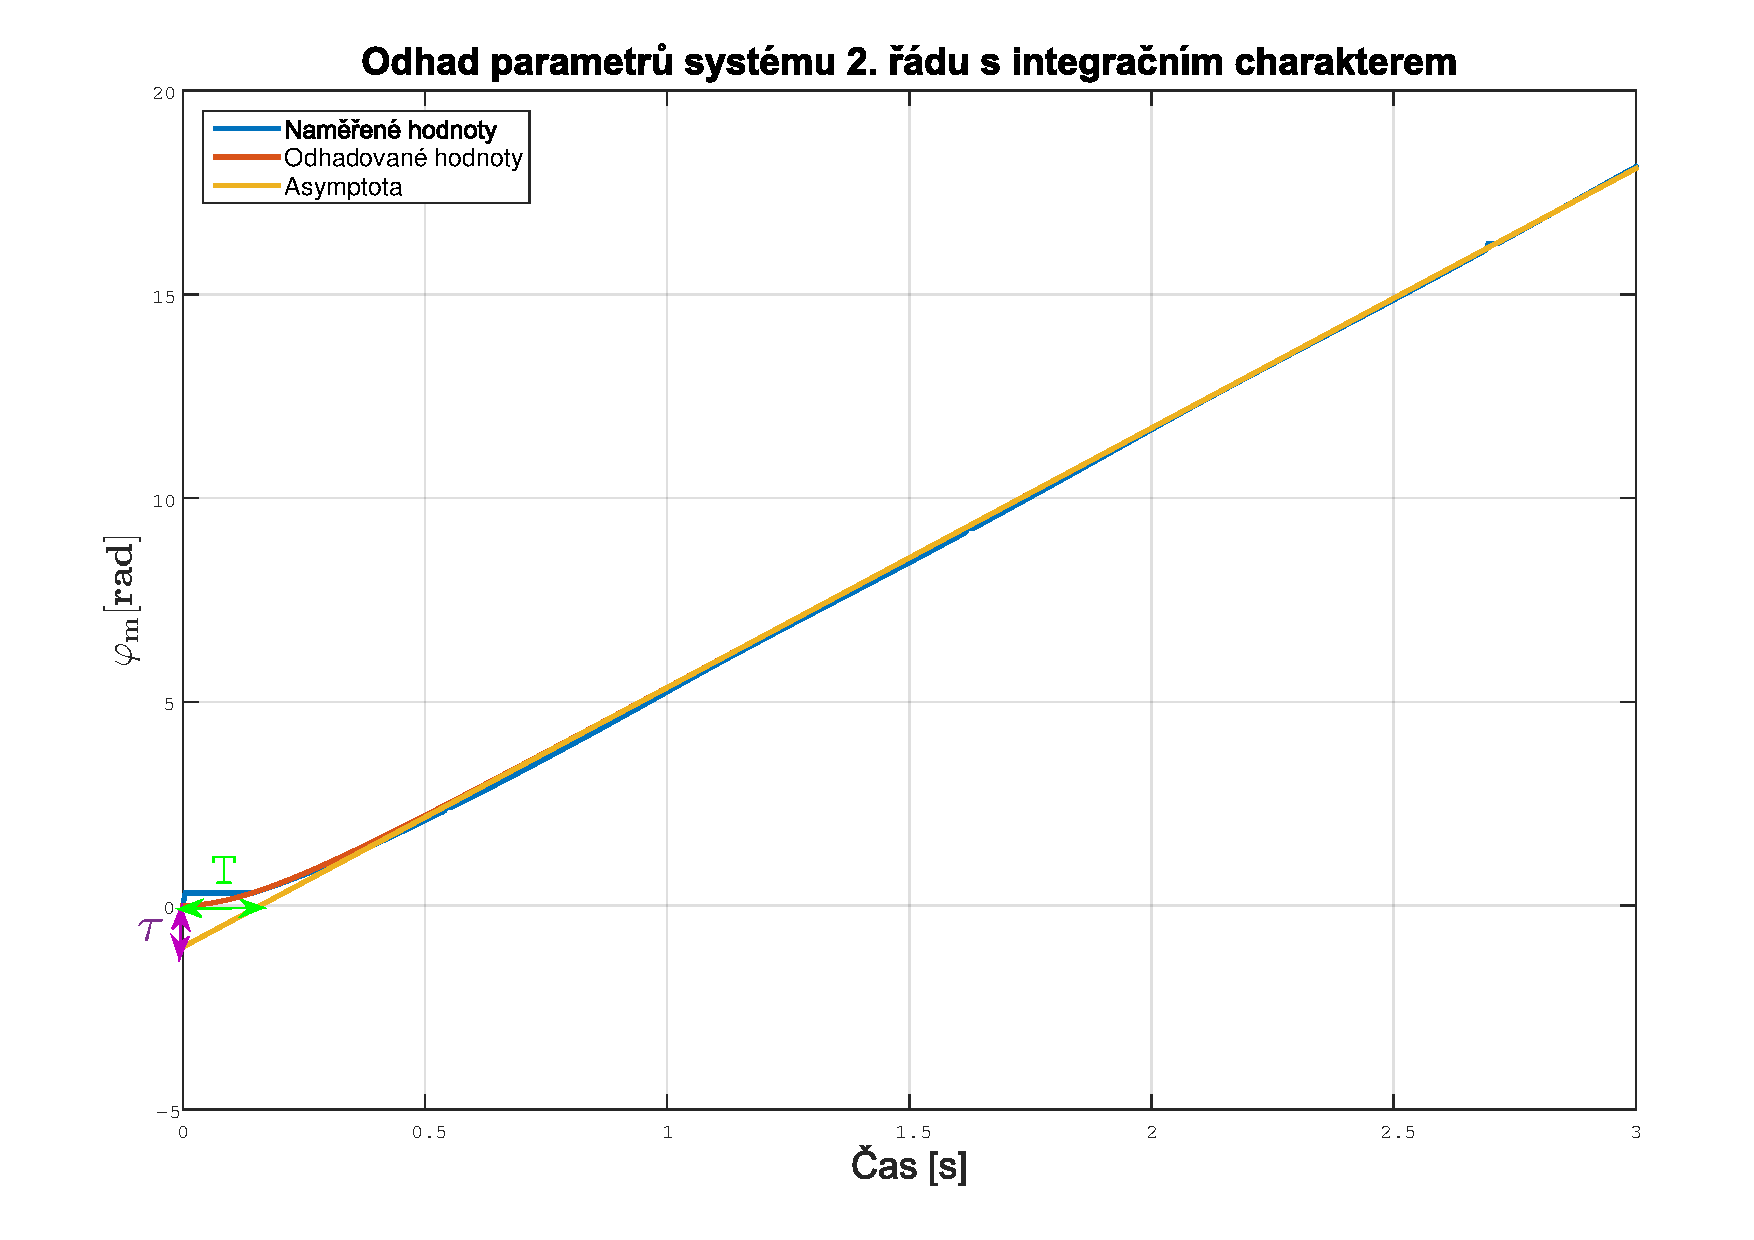
\includegraphics[scale=.4]{Odhad_phim}
    \caption{Odhad parametrů rovnice pro $\varphi_m$ z asymptoty}
\end{figure}

%Matouš-konec%%%%%%%%%%%%%%%%%%%%%%%%%%%%%%%%%%%%%%%%

%Tomáš%%%%%%%%%%%%%%%%%%%%%%%%%%%%%%%

\section{Identifikace dynamiky kyvadla}
Při identifikaci dynamiky kyvadla jsme vycházeli z následující diferenciální rovnice:
$$
J_p \phidd{p} + m g l \coss{\phin{p}} - m l r \phidd{m} \sinn{\phin{p}} + 2 \delta \phid{p} = 0
$$
Identifikaci jsme prováděli v pásmu necitlivosti vlivu kyvadla na rameno, tj. křížový člen  $m l r \phidd{m} \sinn{\phin{p}}$ se neprojevoval, z rovnice jej tedy vypustíme. Dále nahradíme $\coss{\phin{p}}$ jeho lineární aproximací v pracovním bodu, což v našem případě je $\phin{p}$. Získaná rovnice je tedy následující:
$$
J_p \phidd{p} + 2 \delta \phid{p} + m g l \phin{p} = 0
$$


Přenos této rovnice z počátečních podmínek je: 
$$
H_{\phin{p}}(s) = \frac{1}{J_p s^2 + 2 \delta s + m g l}
$$
\newcommand{\wn}{\omega_n}
\newcommand{\ut}{\zeta} % útlum
Tento přenos identifikujeme pomocí přenosu druhého řádu ve tvaru s tlumením $\ut$ a přirozenou frekvencí $\wn$. Porovnáním s přenosovou funkcí $H_{\phin{p}}(s)$ dostáváme:
$$
H_{\phin{p}}(s) = \frac{\frac{1}{J_p}}{s^2 + 2 \frac{\delta}{J_p} s + \frac{m g l}{J_p}}
\overset{!}{=} 
\frac{k \wn^2}{s^2 + 2 \wn \ut s + \wn^2}
$$
Z rovnosti je vidět, že: ,$\frac{m g l}{J_p} = \wn^2$, $\frac{\delta}{J_p} = \wn \ut$. %$\frac{1}{J_p} = k \wn^2$
Z nich si vyjádříme neznámé, které cheme získat, tedy $J_p = \frac{m g l}{\wn^2}$ a $\delta = J_p \wn \ut$. $\wn$ a $\ut$ zjistíme identifikací z odezvy na počáteční podmínku, $m = \SI{0,175}{\kg}$ (viz. zadání), $g = \SI{9,81}{\meter \per \second}$ je tíhové zrychlení a $l = \SI{0,17}{\metre}$ (změřená délku kyvadla).

\begin{figure}[H]
	\centering
    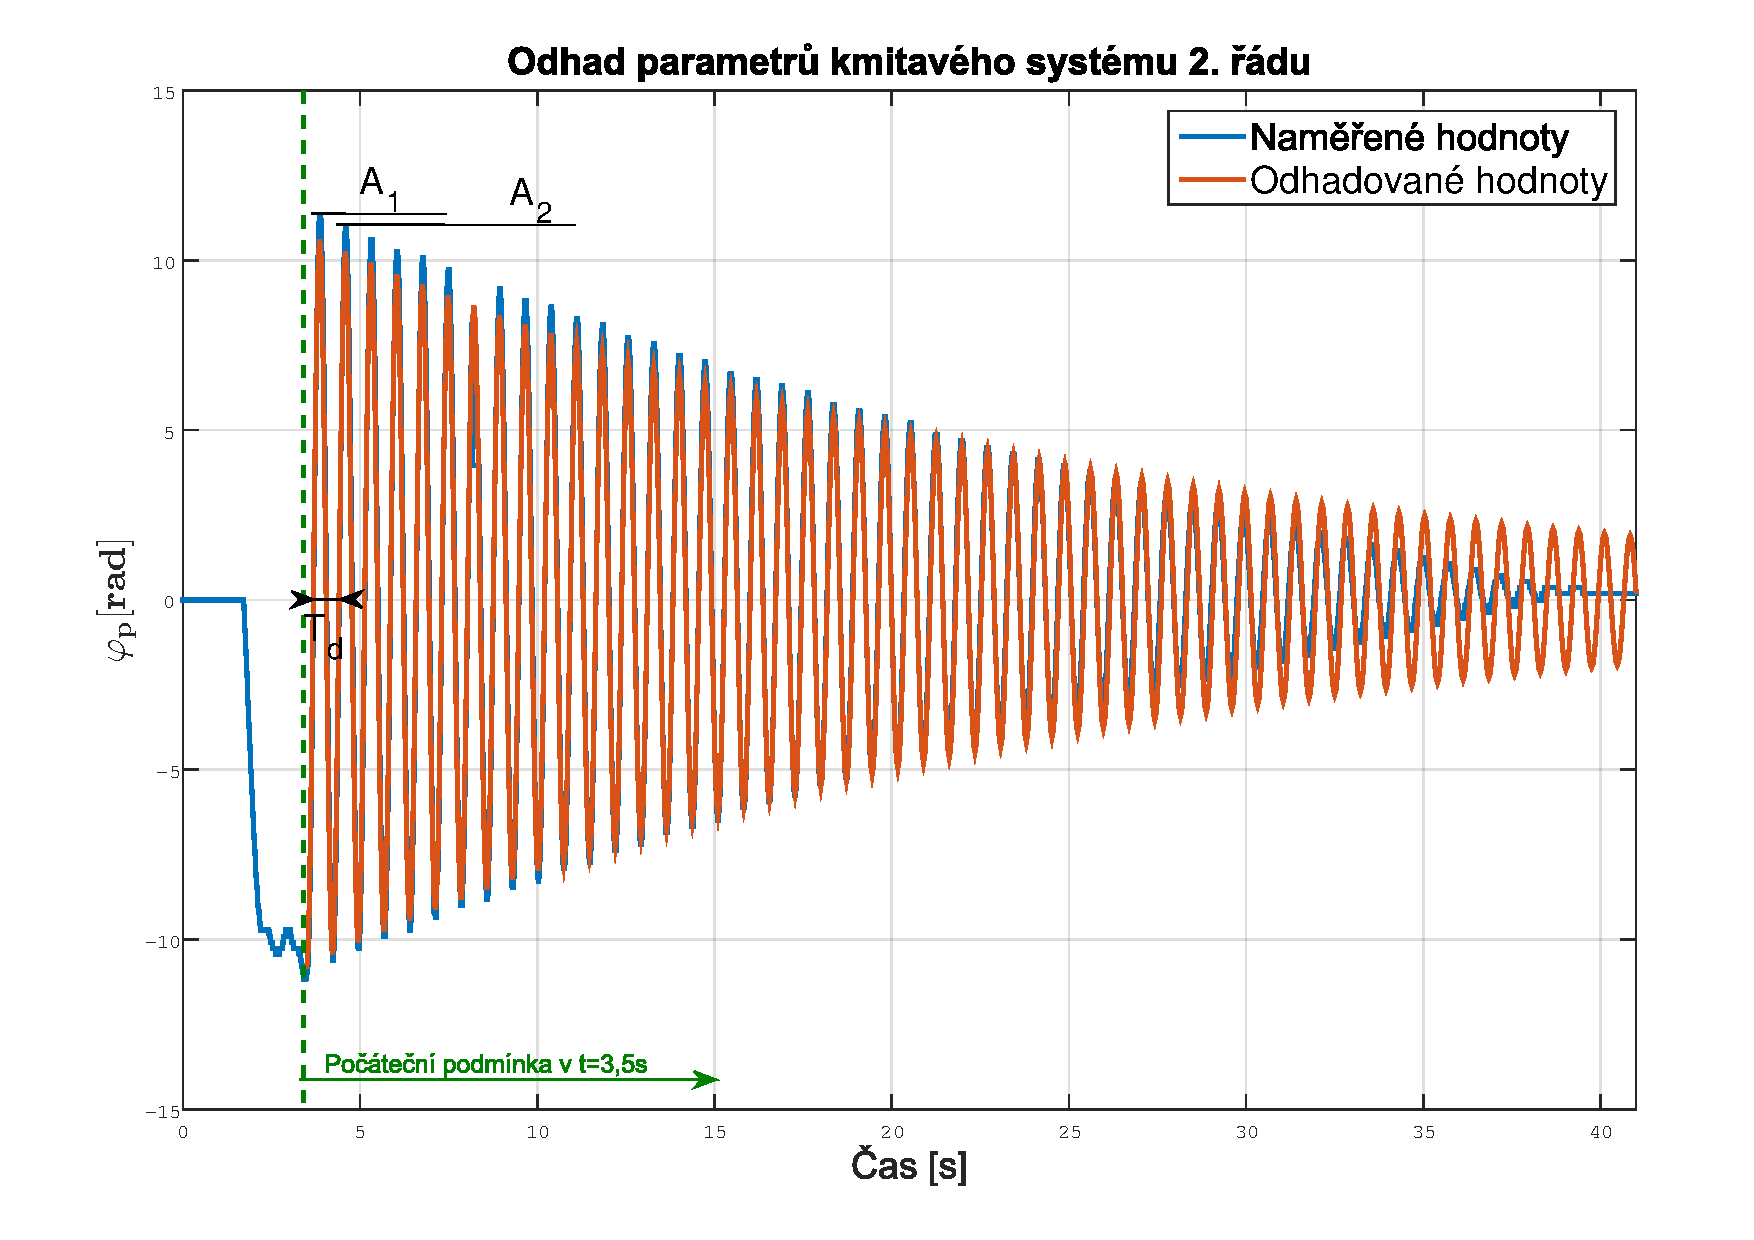
\includegraphics[scale=.6]{Odhad_phip.pdf}
    \caption{Odezva ramene na počáteční podmínku}
\end{figure}


Platí, že $\mu \equiv \ln{(\frac{A_1}{A_2})} \doteq 0,0339$, $\ut = \frac{\mu}{\sqrt{4 \pi^2 + \mu^2}} \doteq 0,0054$, $\wn = \frac{2 \pi}{T_d \sqrt{1 - \ut^2}} \doteq 8,6666$. Dosazením těchto hodnot můžeme tedy získat, že $J_p = \frac{m g l}{\wn^2} \doteq \SI{0.0039}{\kilo \gram \metre \per \second \squared}$, $\delta = J_p \wn \ut \doteq \SI{1.8169e-04}{\kg \m \squared \per \second}$.

%Tomáš-konec%%%%%%%%%%%%%%%%%%%%%%%%%%%%%%%

%Matouš%%%%%%%%%%%%%%%%%%%%%%%%%%%%%%%%%%%%%%%%

\section{Identifikace křížových členů}
Zbývá nám ještě určit konstanty $k_2$ a $k_3$, které v rovnicích tvoří koeficienty křížových členů. Platí, že
\begin{align*}
&k_2 = mlr && k_3 = mgl
\end{align*}
Prvky $l$ a $r$ jsme určili naměřením na modelu kyvadla (jedná se o délku kyvadla a délku ramene), $g$ je tíhové zrychlení, které je pro naši polohu známé, a nakonec hodnotu $m$ jsme dostali zadanou. Výsledné hodnoty tedy jsou:
\begin{align*}
&m = \SI{0,175}{ \kilo \gram} &&g = \SI{9,81}{\meter \per \second}	\\
&l = \SI{0,17}{\meter} &&r = \SI{0,2}{\meter}
\end{align*}

%Matouš - konec %%%%%%%%%%%%%%%%%%%%%%%%%%%%%%%%%%%%%%%%

\section{Provnání odezvy skutečného systému s odezvami linearizovaného a nelinearizovaného modelu}

\begin{figure}[H]
\centering
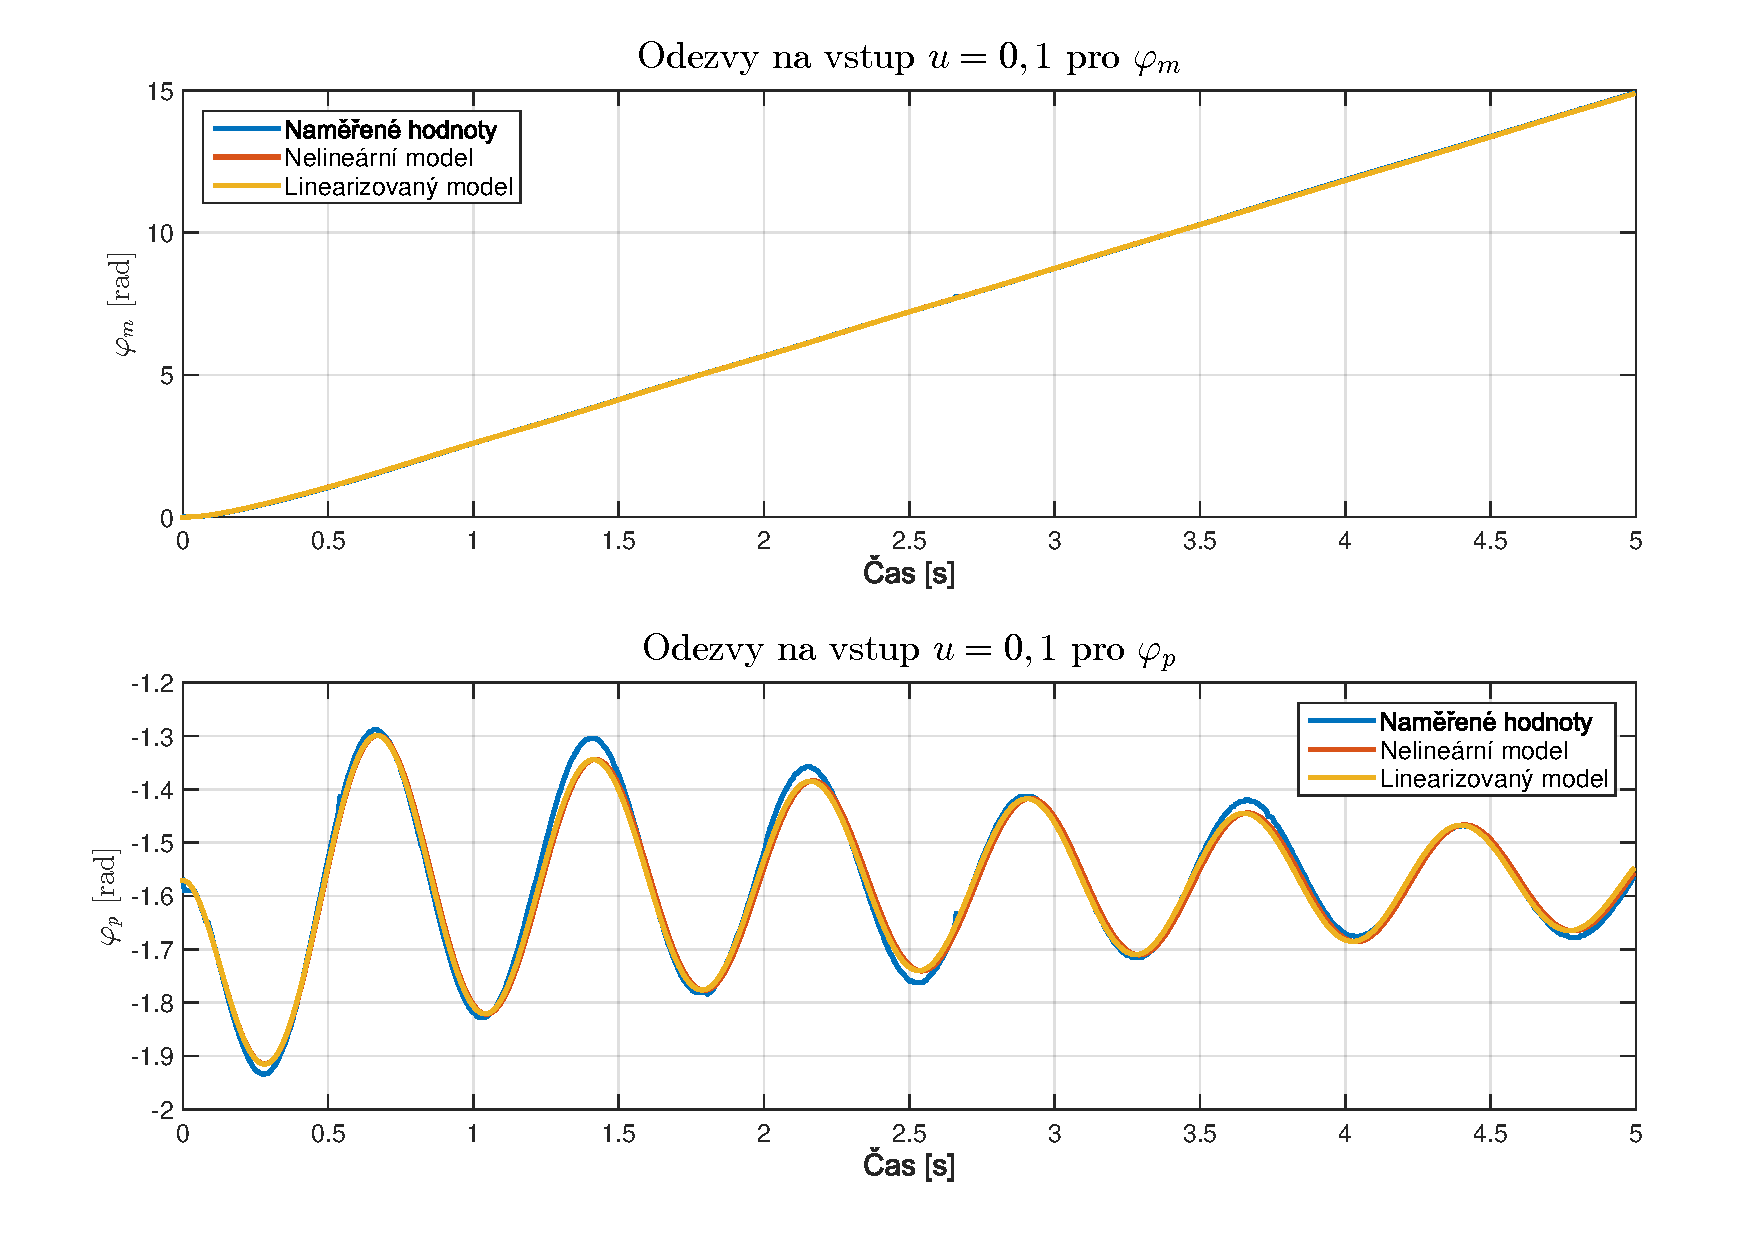
\includegraphics[scale=0.6]{Odezvy01.pdf}
\caption{•}
\end{figure}

\begin{figure}[H]
\centering
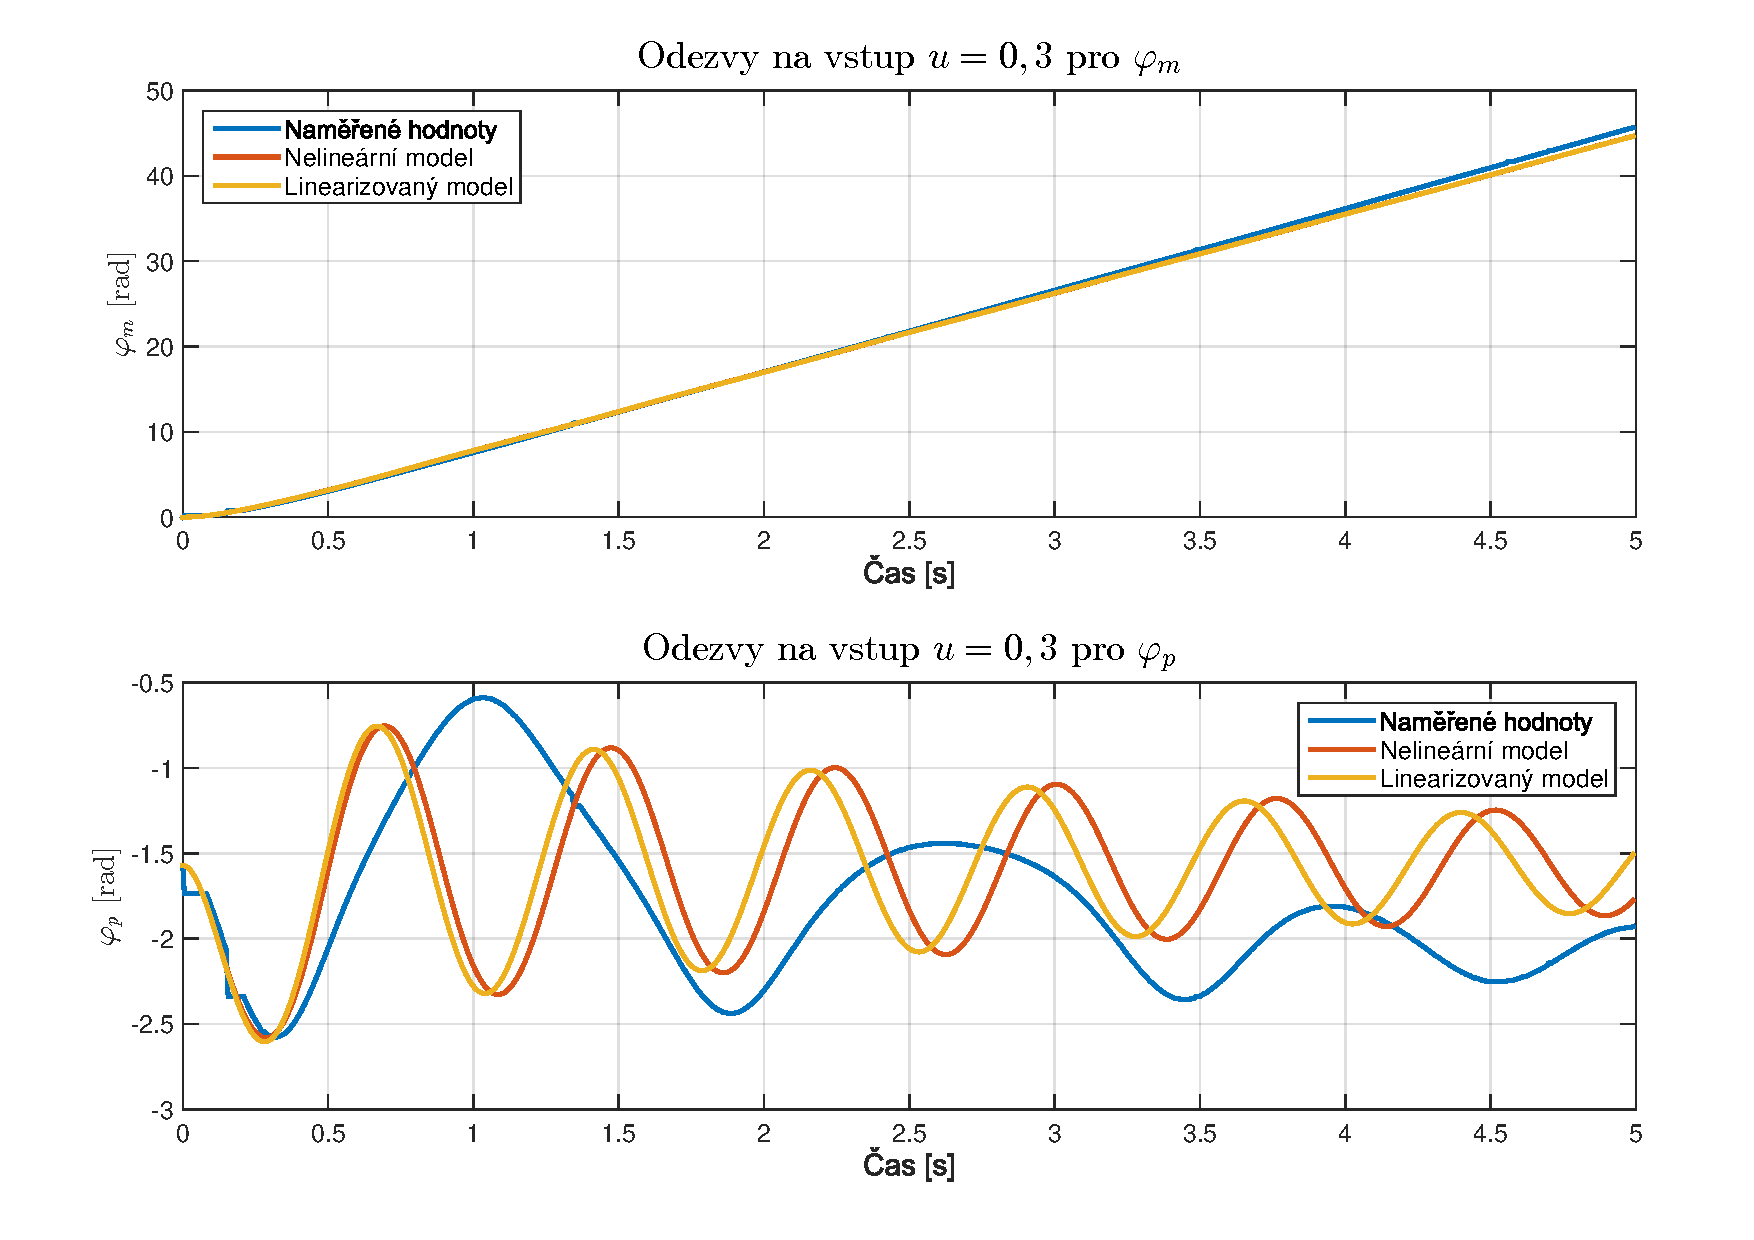
\includegraphics[scale=0.6]{Odezvy03.pdf}
\caption{•}
\end{figure}


\end{document}